\begin{figure}[H]
\centering
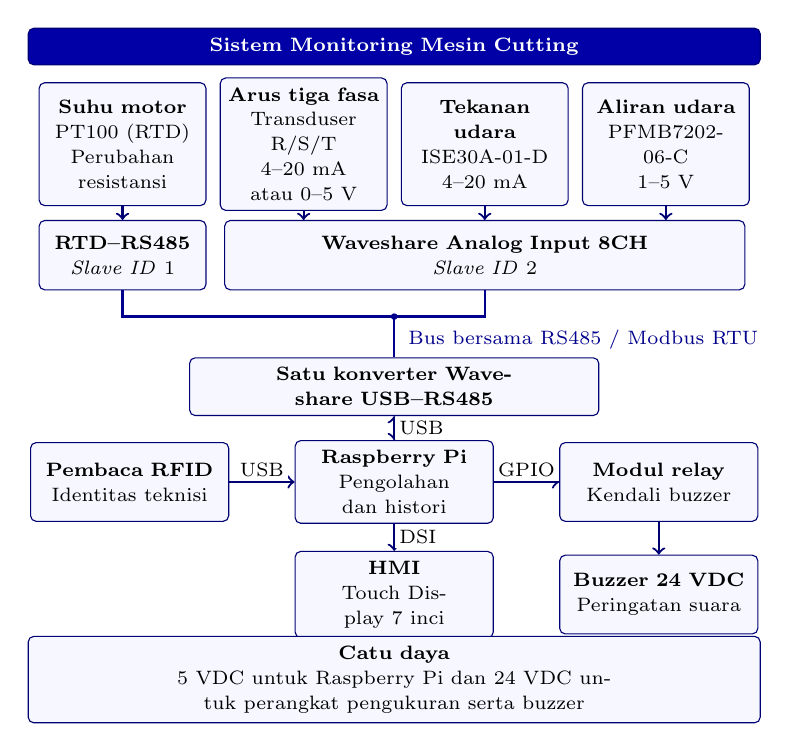
\begin{tikzpicture}[
  font=\rmfamily\fontsize{7.5}{9}\selectfont,
  bloc/.style={draw=blue!45!black,rounded corners=2pt,align=center,
    fill=blue!3,inner sep=3.5pt,text width=4.15cm},
  banner/.style={bloc,fill=blue!65!black,text=white,text width=9.05cm},
  sensor/.style={bloc,text width=1.95cm,inner xsep=2.4pt,minimum height=1.56cm},
  converter/.style={bloc,minimum height=0.88cm},
  device/.style={bloc,text width=2.27cm,minimum height=1cm},
  link/.style={->,thick,draw=blue!45!black},
  bus/.style={thick,draw=blue!55!black},
  tag/.style={font=\rmfamily\fontsize{7}{8}\selectfont,fill=white,inner sep=1.5pt}
]
\node[banner] at (0,0) {\textbf{Sistem Monitoring Mesin Cutting}};
\node[sensor] (suhu) at (-3.45,-1.24)
  {\textbf{Suhu motor}\\PT100 (RTD)\\Perubahan resistansi};
\node[sensor] (arus) at (-1.15,-1.24)
  {\textbf{Arus tiga fasa}\\Transduser R/S/T\\4--20 mA atau 0--5 V};
\node[sensor] (tekanan) at (1.15,-1.24)
  {\textbf{Tekanan udara}\\ISE30A-01-D\\4--20 mA};
\node[sensor] (aliran) at (3.45,-1.24)
  {\textbf{Aliran udara}\\PFMB7202-06-C\\1--5 V};
\node[converter,text width=1.95cm,inner xsep=2.4pt] (rtd) at (-3.45,-2.65)
  {\textbf{RTD--RS485}\\\textit{Slave ID} 1};
\node[converter,text width=6.36cm] (analog) at (1.15,-2.65)
  {\textbf{Waveshare Analog Input 8CH}\\\textit{Slave ID} 2};
\draw[link] (suhu) -- (rtd);
\foreach \inputnode in {arus,tekanan,aliran}
  \draw[link] (\inputnode.south) -- (\inputnode.south |- analog.north);
\draw[bus] (rtd.south) |- (0,-3.43) -| (analog.south);

\node[bloc,text width=4.95cm] (adapter) at (0,-4.32)
  {\textbf{Satu konverter Waveshare USB--RS485}};
\draw[bus] (0,-3.43) -- (adapter.north);
\fill[blue!55!black] (0,-3.43) circle (1.2pt);
\node[tag,right,text=blue!55!black] at (0.12,-3.72)
  {Bus bersama RS485 / Modbus RTU};
\node[device] (pi) at (0,-5.53) {\textbf{Raspberry Pi}\\Pengolahan dan histori};
\draw[link,<->] (adapter) -- node[right,tag]{USB} (pi);
\node[device] (rfid) at (-3.36,-5.53) {\textbf{Pembaca RFID}\\Identitas teknisi};
\node[device] (relay) at (3.36,-5.53) {\textbf{Modul relay}\\Kendali buzzer};
\draw[link] (rfid) -- node[above,tag]{USB} (pi);
\draw[link] (pi) -- node[above,tag]{GPIO} (relay);
\node[device] (hmi) at (0,-6.96) {\textbf{HMI}\\Touch Display 7 inci};
\node[device] (buzz) at (3.36,-6.96) {\textbf{Buzzer 24 VDC}\\Peringatan suara};
\draw[link] (pi) -- node[right,tag]{DSI} (hmi);
\draw[link] (relay) -- (buzz);
\node[banner,fill=blue!3,text=black] at (0,-8.04)
  {\textbf{Catu daya}\\5 VDC untuk Raspberry Pi dan 24 VDC untuk perangkat pengukuran serta buzzer};
\end{tikzpicture}
\caption{Blok diagram sistem monitoring mesin cutting}
\label{fig:draft-3-1}
\end{figure}
